%---------------------------------------------------------------------------%
%-                                                                         -%
%-                           LaTeX Template                                -%
%-                                                                         -%
%---------------------------------------------------------------------------%
%- Copyright (C) Huangrui Mo <huangrui.mo@gmail.com> 
%- This is free software: you can redistribute it and/or modify it
%- under the terms of the GNU General Public License as published by
%- the Free Software Foundation, either version 3 of the License, or
%- (at your option) any later version.
%---------------------------------------------------------------------------%
%->> Document class declaration
%---------------------------------------------------------------------------%
\documentclass[twoside]{Style/ucasthesis}%
%- Multiple optional arguments:
%- [<oneside|twoside|print>]% oneside eprint, twoside eprint, or paper print
%- [fontset=<adobe|none|...>]% specify font set instead of automatic detection
%- [scheme=plain]% thesis writing of international students
%- [draftversion]% show draft version information
%- [standard options for ctex book class: draft|paper size|font size|...]%
%---------------------------------------------------------------------------%
%->> Document settings
%---------------------------------------------------------------------------%

\usepackage[super,list,table,math]{Style/artratex}
%- usage: \usepackage[option1,option2,...,optionN]{artratex}
%- Multiple optional arguments:
%- [bibtex|biber]% set bibliography processor and package
%- [<numbers|super|authoryear|alpha>]% set citation and reference style
%- <numbers>: textual: Jones [1]; parenthetical: [1]
%- <super>: textual: Jones superscript [1]; parenthetical: superscript [1]
%- <authoryear>: textual: Jones (1995); parenthetical: (Jones, 1995)
%- <alpha>: textual: not available; parenthetical: [Jon95]
%- [geometry]% reconfigure page layout via geometry package
%- [lscape]% provide landscape layout environment
%- [xhf]% disable header and footer via fancyhdr package
%- [color]% provide color support via xcolor package
%- [background]% enable page background
%- [tikz]% provide complex diagrams via tikz package
%- [table]% provide complex tables via ctable package
%- [list]% provide enhanced list environments for algorithm and coding
%- [math]% enable some extra math packages
%- [xlink]% disable link colors
\usepackage{Style/artracom}% user defined commands
%---------------------------------------------------------------------------%
%->> Document inclusion
%---------------------------------------------------------------------------%
%\includeonly{Tex/Chap_1,...,Tex/Chap_N}% selected files compilation
%---------------------------------------------------------------------------%
%->> Document content
%---------------------------------------------------------------------------%
%-
%-> Titlepage information
%-

%- ------------- 文前 ----------------
%-> Frontmatter: 
%   封面, 摘要, 全文目录及图表目录, 符号表
%-
%---------------------------------------------------------------------------%
%->> Titlepage information
%---------------------------------------------------------------------------%
%-
%-> 中文封面信息
%-
\confidential{}% 密级:涉密论文或延迟公开论文填写
\schoollogo[scale=0.095]{ucas_logo}% 校徽
\title{面向 DIMM 近存计算系统的调度关键技术研究}% 论文中文题目
\author{潘炤伍}% 论文作者
\advisor{张佩珩~正研级高级工程师\\~中国科学院计算技术研究所}% 指导教师:姓名 专业技术职务 工作单位
%\advisor{指导教师一\\指导教师二\\指导教师三}% 多行指导教师示例
\degree{硕士}% 学位:学士、硕士、博士
\degreetype{工学}% 学位类别:理学、工学、工程、医学等
\major{计算机系统结构}% 一级/二级学科专业名称,领域名称需要与学籍信息一致
\institute{中国科学院计算技术研究所}% 院系名称
%\institute{中国科学院力学研究所\\流固耦合实验室}% 多行院系名称示例
\date{2024~年~6~月}% 毕业日期:夏季为6月、冬季为12月
%-
%-> 英文封面信息
%-
\TITLE{Research on Scheduling Techniques for Near-Memory Computing Targeting real PIM system with PIM-DIMMs}% 论文英文题目
\AUTHOR{Zhaowu Pan}% 论文作者
\ADVISOR{Supervisor: Professor Peiheng Zhang}% 指导教师
\DEGREE{Master}% 学位:Bachelor, Master, Doctor, Postdoctor。封面据英文学位名称自动切换,需确保拼写准确
\DEGREETYPE{Engineering}% 学位类别:Philosophy, Natural Science, Engineering, Economics, Agriculture 等
\MAJOR{Computer Architecture}% 二级学科专业名称
\INSTITUTE{Institute of Computing Technology, Chinese Academy of Sciences}% 院系名称
\DATE{June, 2024}% 毕业日期:夏季为June、冬季为December
%---------------------------------------------------------------------------%
% 论文相关个人及其他信息
\begin{document}

\frontmatter
%---------------------------------------------------------------------------%
%->> Frontmatter
%---------------------------------------------------------------------------%
%-
%-> 生成封面
%-

\maketitle% 生成中文封面
\MAKETITLE% 生成英文封面
%-
%-> 作者声明
%-
\makedeclaration% 生成声明页
%-
%-> 中文摘要
%-
\intobmk\chapter*{摘\quad 要}% 显示在书签但不显示在目录
\setcounter{page}{1}% 开始页码
\pagenumbering{Roman}% 页码符号
在过去的二十年里,随着通用处理器制程和工艺的演进,面对计算密集型负载,近存计算技术是一种用于缓解,整体流程分
,其核心是。xx任务具有...,...,...的问题,目前的
,其...有待提升。同时,由于
,因此...对...有一定的要求。本文针对...提
出了基于...的..,通过...等技术在
...设备上进行高效的...,最终实现...且保证...
...的...。本文的主要研究工作以及贡献如下:
本文提出了一种基于...的...MetaPB。首先,
得益于...并行度高的优点,...实现了在...上的
...。其次,在架构设计时,本文基于...
在保证...的同时实现具备...的...,并结合...
...对模型进行改进。为了适应...任务场景,本文设计并实验了高效的
,在 ...模块中使用了...,在...阶段基于...和...技术进行...预测。最终在保证模型效率的情况
下,实现了一个具备较高..的算法模型。

本文在模型和架构层面实现了对...算法的优化。对于模型层面,
在整体框架设计时针对任务的特点引入结构,在模型内
部使用...提高了...效率,最终提高了近存计算系统运行混合负载时的能耗与性能。
为了适应不同...应用场景下对运行能效和性能的需求,在
可接受的...损失条件下,本文使用...技术实现了具备
...模型。在架构层面,本文探索了...技术在...任务场景中的应
用,在不同...下实现了在 ...上的...加速。最终本文联合
和架构的...优化,完成了对...的整体改进。
本文通过上述的算法设计并实现了一个基于...的...
,该模型具备较高的...,同时不同...的模型能够适应
各类...场景。本文提出的...能够用于对...的..进行...,
通过...、...、...和...四个流程,得到具备较
高...的...。经过...个测试...的实验对比,本文提出的 MetaPB
相比于粗粒度CPU-DPU调度在性能优先模式上... 能效模式上...平均获得了...


\keywords{中国科学院大学,学位论文,模板}% 中文关键词
%-
%-> 英文摘要
%-
\intobmk\chapter*{Abstract}% 显示在书签但不显示在目录

Chinese abstracts, English abstracts, table of contents, the main contents, references, appendix, acknowledgments, author's resume and academic papers published during the degree study and other relevant academic achievements must start with another right page (odd-numbered page).
    %- the current style, comment all the lines in plain style definition.

\KEYWORDS{University of Chinese Academy of Sciences, Thesis, LaTeX Template}% 英文关键词

\pagestyle{enfrontmatterstyle}%
\cleardoublepage\pagestyle{frontmatterstyle}%

%---------------------------------------------------------------------------%
% 封面和中英文摘要
\fancypagestyle{figureheader}{
  \fancyhf{}
  \fancyhead[C]{\footnotesize 图表目录}%此处填写中文标题
  \fancyfoot[C]{\footnotesize \thepage}% page number
    \renewcommand{\headrulewidth}{0.8pt}% header rule
    \renewcommand{\footrulewidth}{0pt}% footer rule
}
{% ---- 目录区 ------
\linespread{1.2}% local line space
\intobmk*{\cleardoublepage}{\contentsname}% add link to bookmark
\tableofcontents% content catalog

\intobmk*{\cleardoublepage}{图表目录}
\thispagestyle{noheaderstyle}
{
\renewcommand*{\addvspace}[1]{}
\let\oldnumberline\numberline%
\renewcommand{\numberline}{\figurename~\oldnumberline}%
\listoffigures%
}
{
\let\cleardoublepage\relax
\let\clearpage\relax
\renewcommand*{\addvspace}[1]{}
\let\oldnumberline\numberline%
\renewcommand{\numberline}{\tablename~\oldnumberline}%
\listoftables%
}
 % 图目录
\thispagestyle{figureheader}
}
\intobmk\chapter*{符号列表}% 显示在书签但不显示在目录

\section*{字符}
\nomenclatureitem[\textbf{Unit}]{\textbf{Symbol}}{\textbf{Description}}
\nomenclatureitem[$\Unit{m^{2} \cdot s^{-2} \cdot K^{-1}}$]{$R$}{the gas constant}
\nomenclatureitem[$\Unit{m^{2} \cdot s^{-2} \cdot K^{-1}}$]{$C_v$}{specific heat capacity at constant volume}
\nomenclatureitem[$\Unit{m^{2} \cdot s^{-2} \cdot K^{-1}}$]{$C_p$}{specific heat capacity at constant pressure}
\nomenclatureitem[$\Unit{m^{2} \cdot s^{-2}}$]{$E$}{specific total energy}
\nomenclatureitem[$\Unit{m^{2} \cdot s^{-2}}$]{$e$}{specific internal energy}
\nomenclatureitem[$\Unit{m^{2} \cdot s^{-2}}$]{$h_T$}{specific total enthalpy}
\nomenclatureitem[$\Unit{m^{2} \cdot s^{-2}}$]{$h$}{specific enthalpy}
\nomenclatureitem[$\Unit{kg \cdot m \cdot s^{-3} \cdot K^{-1}}$]{$k$}{thermal conductivity}
\nomenclatureitem[$\Unit{kg \cdot m^{-1} \cdot s^{-2}}$]{$S_{ij}$}{deviatoric stress tensor}
\nomenclatureitem[$\Unit{kg \cdot m^{-1} \cdot s^{-2}}$]{$\tau_{ij}$}{viscous stress tensor}
\nomenclatureitem[$\Unit{1}$]{$\delta_{ij}$}{Kronecker tensor}
\nomenclatureitem[$\Unit{1}$]{$I_{ij}$}{identity tensor}

\section*{算子}
\nomenclatureitem{\textbf{Symbol}}{\textbf{Description}}
\nomenclatureitem{$\Delta$}{difference}
\nomenclatureitem{$\nabla$}{gradient operator}
\nomenclatureitem{$\delta^{\pm}$}{upwind-biased interpolation scheme}

\section*{缩写}
\nomenclatureitem{CFD}{Computational Fluid Dynamics}
\nomenclatureitem{CFL}{Courant-Friedrichs-Lewy}
\nomenclatureitem{EOS}{Equation of State}
\nomenclatureitem{JWL}{Jones-Wilkins-Lee}
\nomenclatureitem{WENO}{Weighted Essentially Non-oscillatory}
\nomenclatureitem{ZND}{Zel'dovich-von Neumann-Doering}

% 符号表

%-
%-> ------------ 正文区----------------
%-
\mainmatter% initialize the environment
\renewcommand{\labelenumi}{(\arabic{enumi}) }
\renewcommand{\labelenumii}{(\arabic{enumi}).\arabic{enumii}}
\renewcommand{\labelenumiii}{(\arabic{enumi}).\arabic{enumii}.\arabic{enumiii}}
\renewcommand{\labelenumiv}{(\arabic{enumi}).\arabic{enumii}.\arabic{enumiii}.\arabic{enumiv}}
%---------------------------------------------------------------------------%
%->> Main content
%---------------------------------------------------------------------------%
\renewcommand{\thefigure}{\thechapter-\arabic{figure}}
\renewcommand{\thetable}{\thechapter-\arabic{table}}
\renewcommand{\theequation}{\thechapter-\arabic{equation}}

\chapter{引言}\label{chap:Introduction}
%%%%%%%%%%%%%%%%%%%%%%%%%%%%%%%%%%%%%%%%%%%%%%%%%%%%%%%%%%%%%%%%%%%%%%
\section{研究背景与意义}\label{sec:background_and_motivation}
    \subsection{存算性能剪刀差与存储墙}\label{subsec:memory_wall}

    随着科技和信息化进程的持续加速,计算技术已经成为支持现代社会发展的关键基石。为了满足不断增长的高性能计算需求以及层出不穷的新型负载,计算机系统结构研究者正面临着一系列挑战。  
    
    在过去的几十年中,受益于集成电路制造工艺和封装技术的飞速演进,通用处理器技术的迭代一直是推动高性能计算系统计算能力增长的中坚力量。然而在如今,尤其是在面对新型高性能计算负载时,如生物信息学、数据库和图计算负载时,主存储器和CPU核心之间的数据搬移在
    延迟\citep{hashemi_accelerating_nodate}和能耗\citep{pandiyan_quantifying_2014}方面都产生了不可忽视的开销,通用处理器正逐渐显露出其架构与生俱来的局限性。此外,如图~\ref{fig:hw_scaling}所示,处理器与存储器在发展中性能所形成的“剪刀差”,加剧了计算过程中由数据搬移所形成的访存瓶颈,构成了通用计算系统能耗的显著比重\citep{denning_exponential_2016}。该现象早在上世纪末就被研究者广泛地意识到,此后被相关领域研究者统称为存储墙(Memory Wall)\citep{wulf_hitting_1995}问题。而随着此前通用处理器发展所遵循的摩尔定律\citep{moore_cramming_1998}和丹纳德缩放定律\citep{dennard_design_nodate}在二十世纪初的先后放缓或失效,处理器的功耗随其运行频率的增长而急剧增加,这也限制了单一处理器计算密度和规模的进一步提升。对冯诺依曼体系结构下的新型计算机系统结构、乃至非冯诺依曼体系结构的设计,已经成为诸多高性能计算系统工作的焦点。
    
    \begin{figure}[!htbp]
        \centering
        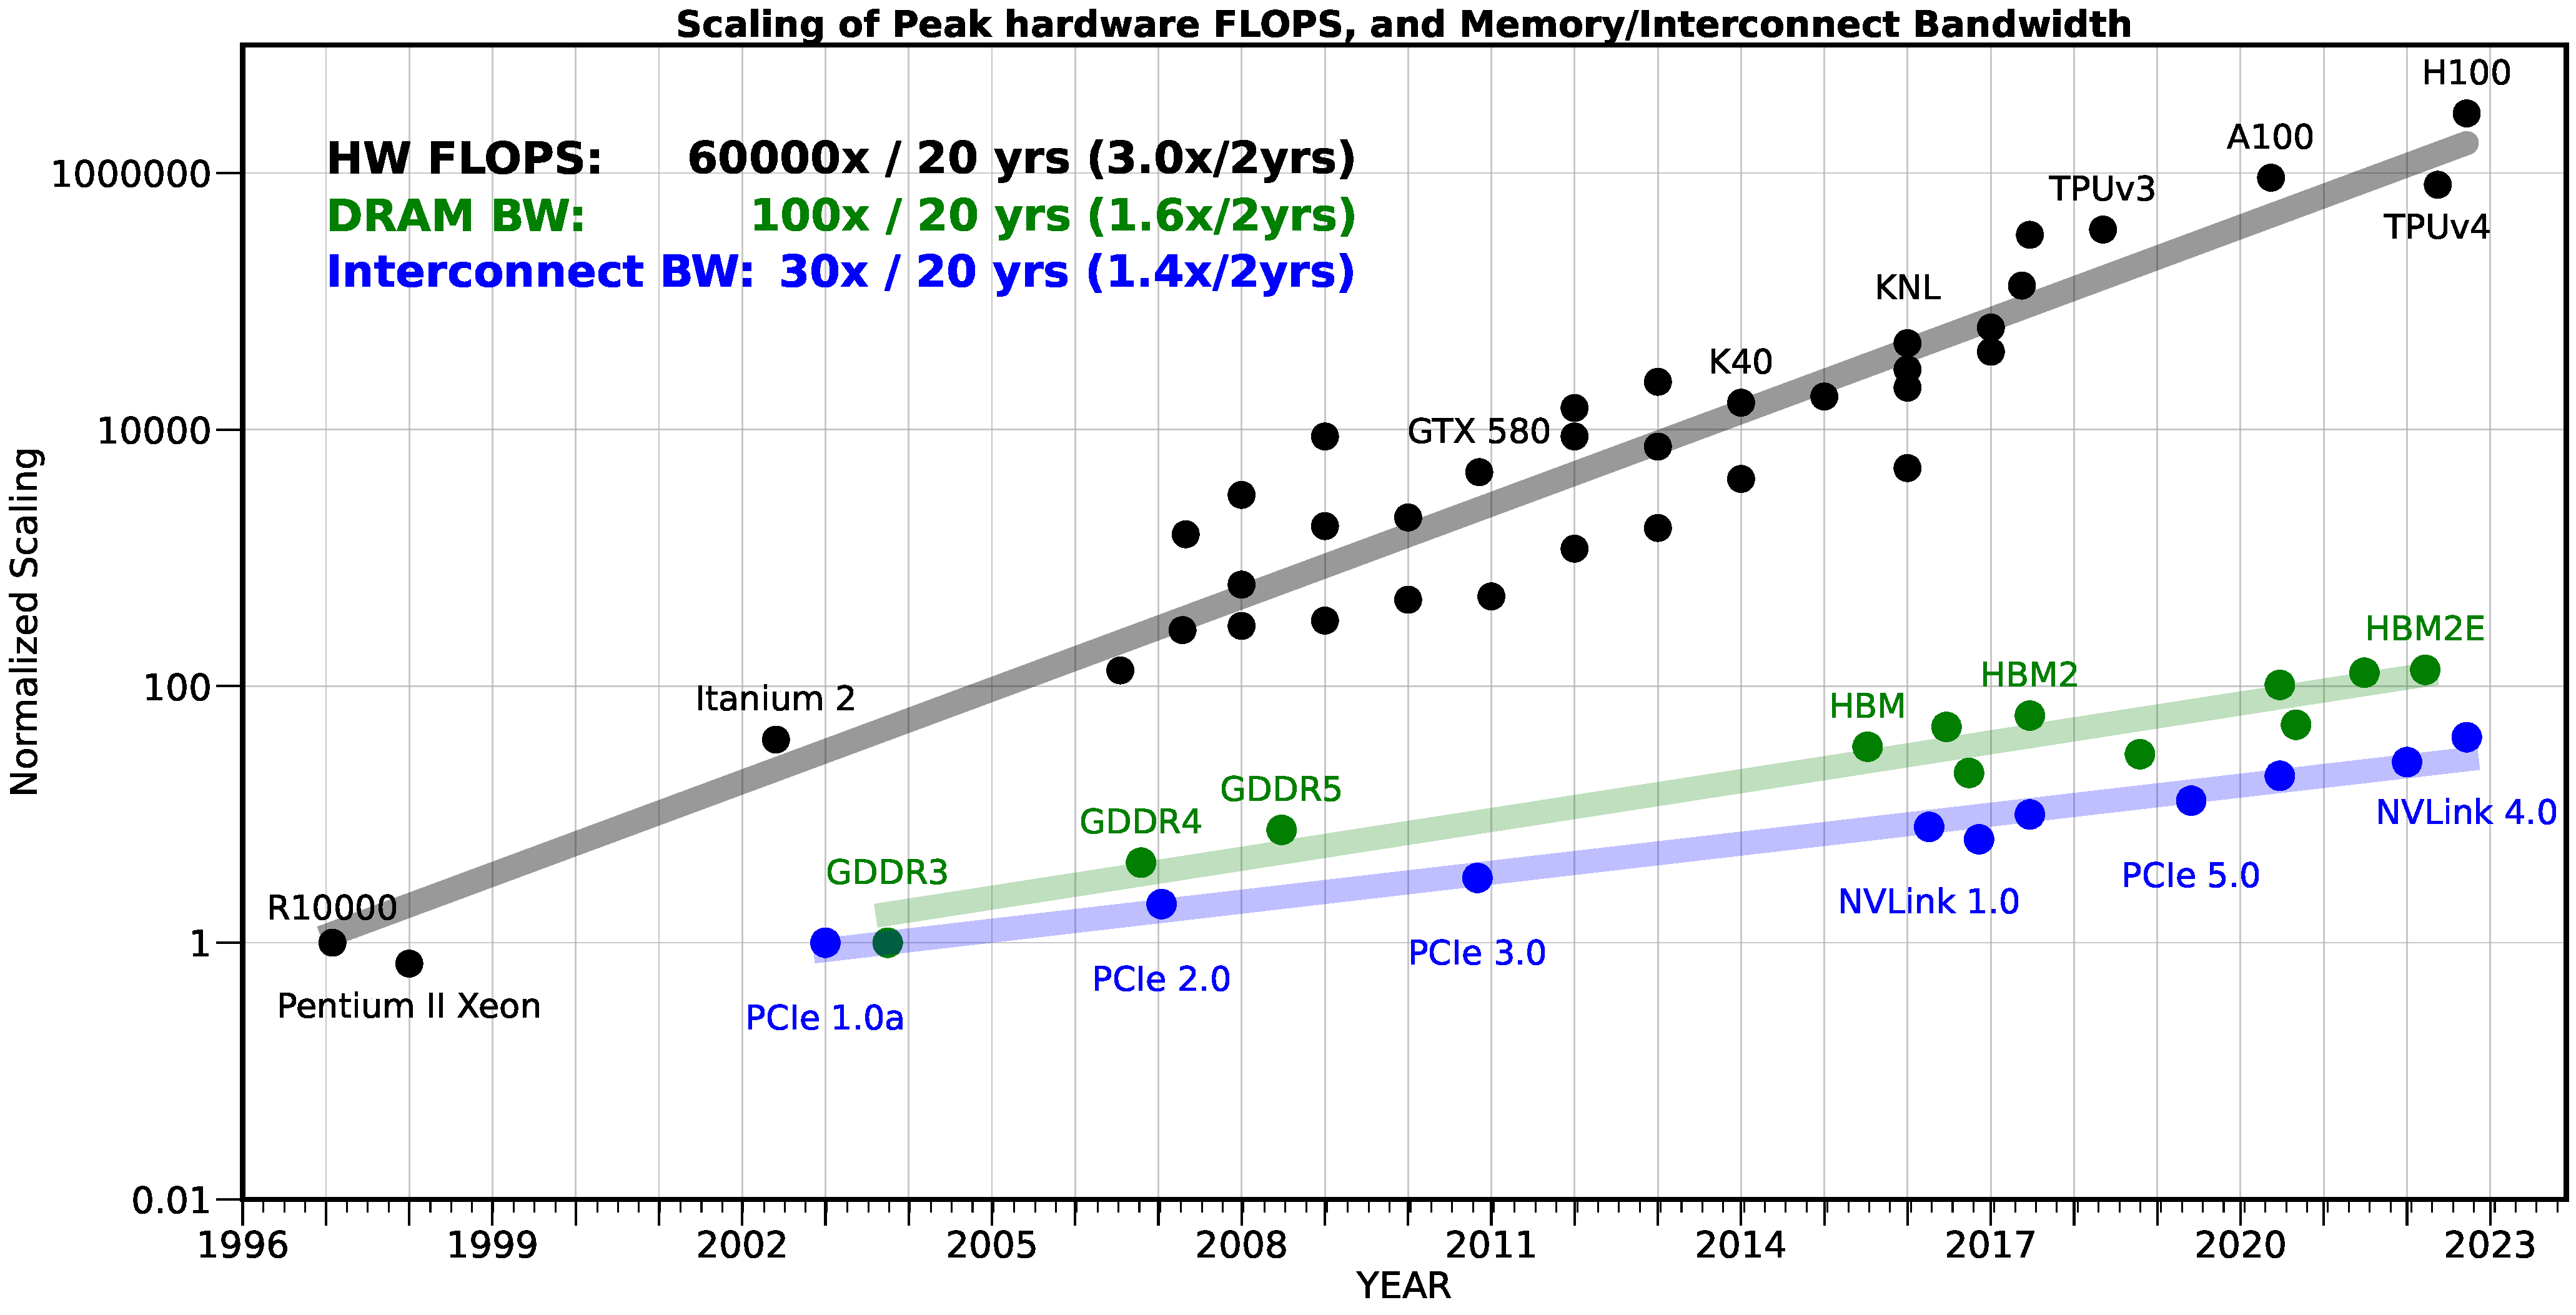
\includegraphics[width=0.85\textwidth]{hw_scaling}
        \bicaption{\quad 计算-存储-互联性能剪刀差示意图\citep{gholami_ai_2023}}
        {\quad Illustration of Compute-DRAM-Interconnect performance gap\citep{gholami_ai_2023}}
        \label{fig:hw_scaling}
    \end{figure}
    
    在高性能计算领域,许多工作负载之所以面临“存储墙”问题,根本原因在于处理器在执行某些计算密集型任务时,必须频繁地通过高延迟、低带宽的内存总线进行数据搬移。这些任务往往具有较差的时间-空间局部性,其中的数据复用不足以抵消或分摊主存储器访问的时间成本。随着存储和计算单元在延迟和带宽上的差距日益扩大,数据搬移导致的性能瓶颈在高性能计算任务中变得日益显著。

    在稀疏矩阵计算中,矩阵数据展现的不同稀疏模式以及采用的矩阵压缩方式对算法性能都有着显著的影响。这类算法普遍具有大量随机访存特性,因此其性能在很大程度上受到访存性能的限制。
    
    在生物信息学领域,基因序列比对和变异分析是关键的计算负载。当前被广泛使用的二代基因测序技术能够在一次全基因测序中产生总量高达数十甚至数百GB的基因读序,这些读序长度通常为数百个字符。在考虑多种变异的情况下,将这些读序精确地比对到共有数十亿碱基对的人类基因组中,是对存储系统性能的严峻挑战。序列比对过程中几乎不涉及密集的浮点运算和整数乘除法,而是涉及大量位运算和整数加减法,伴随着大跨度、随机性强、局部性差的访存模式。

    在数据库领域,关系型数据库中的join操作是一种出现频率高且十分耗时的操作。由于涉及多个表的数据操作、复杂的连接条件以及数据分布的不均匀性,尽管这类操作易于书写和理解,其性能问题却一直广受诟病。因此,对这类操作的规避和等价替换成为提升数据库性能的常见策略。
    
    \subsection{近存计算技术的发展}\label{subsec:evolution_of_PNM}
    为了从根本上缓解数据搬移开销所带来的访存瓶颈,另一种计算范式走上了历史舞台,这种范式通过把计算能力“下放”给主存储器模块,从而使其在计算中发挥主动作用。
    
    在狭义上,区别于是否真正对内存的硬件结构做出修改,该范式中的一部分实现被称为“近存计算”(Processing-Near-Memory,PNM),但其通常也与另一类实现——“可计算存储”(Processing-Using-Memory, PUM)被统称为广义上的“存内计算”(Processing-In-Memory, PIM):前者在存储单元附近集成计算逻辑,如\citep{chang_energy-efficient_2021}\citep{fernandez_natsa_2020}后者直接改变存储单元物理结构以使得其拥有计算能力,如\citep{tu_multcim_2023}\citep{zhang_edge_2023},区别于设计理念与具体的技术实现,广义的存内计算概念可以按表~\ref{tab:PIM-category}分为若干类别

    \begin{table}[!htbp]
        \bicaption{\quad 存内计算范式的设计理念与技术实现}{\quad PIM Approaches and Technologies}
        \label{tab:PIM-category}
        \centering
        \footnotesize% fontsize
        \setlength{\tabcolsep}{4pt}% column separation
        \renewcommand{\arraystretch}{1.2}%row space 
        \begin{tabular}{cl}
            \hline
            设计理念 & 技术实现\\
            %\cline{2-9}% partial hline from column i to column j
            \hline
            可计算存储 (PUM)&\begin{tabular}{l}
                                    基于SRAM\\
                                    基于DRAM\\
                                    基于相变内存(Phase-change memory, PCM)\\
                                    基于磁记忆体(Magnetic RAM, MRAM)\\
                                    基于忆阻器(Resistive RAM, RRAM)
                                    \end{tabular}\\
            \hline
            近存计算 (PNM)&\begin{tabular}{l}
                                    基于3D堆叠内存中的逻辑层\\
                                    基于硅中介层(Silicon interposers)附加逻辑\\
                                    基于近内存控制器附加逻辑\\
                                    基于近内存颗粒附加逻辑\\
                                    基于近内存模块附加逻辑\\
                                    基于近缓存附加逻辑\\
                                    基于近储存设备附加逻辑
                                    \end{tabular}\\
            \hline
        \end{tabular}
    \end{table}
    
    其中,近存计算技术的核心思想是将通过向存储单元附近集成计算元件,将计算能力下放到内存系统中,以减少数据在主存储器和CPU之间的频繁移动,从而在访存密集型工作负载运行时降低延迟和能源消耗\citep{mutlu_modern_2022}。而本课题所涉及到的基于DIMM的近存计算技术则是对现有的DIMM内存模块进行定制,将计算能力集成在内存颗粒之中,从而实现近存计算。通过将计算与内存紧密结合,PIM技术有望从根本上均摊计算访存强度不匹配时数据移动的开销,从而改善内存密集型工作负载的性能。
    
    由于以UPMEM为主的众多近存计算系统在相当多的文献中将自己所属的范式归类为“存内计算(PIM)”,本文为了在简洁的同时避免“大端小端”式的混淆,后续所提到的“PIM”及“存内计算”,若未特别指出,均指的是Processing-Near-Memory, 即特指“近存计算”。
    
    \subsection{近存计算技术所面临的挑战}\label{subsec:challenge_for_PNM}
    近存计算系统作为一种特殊的系统结构,在面对访存瓶颈负载时拥有得天独厚的优势。然而,在该技术应用于现实的计算机系统时,仍存在着较多共同的问题和挑战:
    \begin{enumerate}
        \item 与现有计算机硬件系统的集成
        \item 工具链与软件生态的完善
        \item 近存负载的划分与调度
        \item 软硬协同设计的高性能算子实现
    \end{enumerate}
%%%%%%%%%%%%%%%%%%%%%%%%%%%%%%%%%%%%%%%%%%%%%%%%%%%%%%%%%%%%%%%%%%%%%%
\section{国内外研究现状}\label{sec:related_researches}
    \subsection{近存计算技术研究与应用}
     近些年来,诸多有关近存计算架构的研究和实现都致力于降低计算和存储单元间的物理距离、提升两者间的通信带宽\citep{devaux_true_2019,
     kwon_254_2021,
     ke_near-memory_2022,
     lee_hardware_2021,
     lee_1ynm_2022,
     niu_184qpsw_2022},从而降低能耗并提高吞吐率以及对数据局部性的利用能力,而基于DIMM的近存计算技术主要致力于在内存颗粒附近集成计算逻辑,基于成熟的内存工艺与技术来实现近存计算,是诸多近存计算技术方案中通用性最强、落地最快的一支\citep{mutlu_modern_2022}。
    
    其中,AxDIMM\citep{ke_near-memory_2022} 在DRAM ranks附近放置了一个FPGA,用于加速推荐系统中的机器学习算子以及数据库操作\citep{lee_improving_2022}。通过实现存内加速计算(acceleration mode)和直通(non-acceleration mode)两种模式来进行计算中设备运行逻辑转换。
    
    Samsung FIMDRAM\citep{kwon_254_2021} 在High Bandwidth Memory(HBM)\citep{jun_hbm_2017}的bank附近配备了向量处理单元,是专门为深度学习应用而设计的一类近存计算系统。相似地,SK Hynix AiM\citep{lee_1ynm_2022} 也是一种专为深度学习负载而设计的近存计算系统。该解决方案在每一颗GDDR6存储颗粒附近放置了一颗1GHz,峰值浮点运算能力32GFLOPS的向量处理单元,用于处理RNN和MLP负载。
    
    Alibaba HB-PNM\citep{niu_184qpsw_2022}的实现中,将一层DRAM和一个带有用于加速推荐系统的处理单元的逻辑层通过双层3D堆叠(非多层TSV)的方式粘合在一起,并在逻辑层中加入用于处理深度学习相关的领域专用加速器。在实际商业化推荐模型的运行中获得了相对于CPU-DRAM系统9.78倍的加速,317.43倍的能耗比以及同芯片面积下约660倍的推理算力。
    
    特别地,本项工作中所使用的UPMEM PIM系统\citep{devaux_true_2019}是截至本文书写时(2024年3月)市面上为数不多的使用存内计算架构的商用计算系统,它在传统DIMM内存颗粒上都集成了低功耗的、基于RISC-V架构的通用处理核心UPMEM-DPU,在\citep{gomez-luna_benchmarking_2021}。
    
    与前面所介绍的几种近存计算的模式类似,UPMEM PIM 系统的实现中不涉及到对存储单元硬件结构的修改,而是在存储单元附近集成运算逻辑。但区别于前面介绍的几项的工作,UPMEM PIM系统为每一颗内存颗粒上集成的是一个可以独立处理运算和控制流的、完整功能的RISC-V核心,且不同于AxDIMM的两种模式(“加速器模式”和“直通模式”),UPMEM-DIMM的内存空间不可被宿主机直接访问,因此在实际的编程和使用中往往是被当做异构外部设备看待的。所以,涉及到基于UPMEM PIM-DIMM调度相关的研究时,对异构负载调度相关工作的参考是具有必要的。 

    目前,UPMEM PIM系统在生物信息学\citep{diab_framework_2023,
                                        abecassis_gapim_2023,
                                        diab_high-throughput_2022}、
                        数据库\citep{kang_pim-tree_2022, 
                                    bernhardt_pimdb_2023,
                                    lim_design_2023}、
                        机器学习\citep{gomez-luna_machine_2022,
                                    das_implementation_2022,
                                    gomez-luna_experimental_2023}以及
                        稀疏矩阵运算\citep{giannoula_sparsep_2022}
                        等领域都有相关的应用,并获得了出色的加速比和能效比,展现出了较强的实际应用价值。

    \subsection{异构调度技术研究与应用}\label{subsec:hetero_scheduling_intro}
     异构计算系统负载调度问题一直是一个受学术界和工业界广泛关注的问题。近年来,随着云计算、分布式计算技术以及异构计算技术的并肩发展,集成异构处理器的云服务器以及分布式异构集群的实践层出不穷。异构系统的负载调度对于整个系统的吞吐量和能耗比有着至关重要的作用,但区别于传统的负载均衡算法,在为异构计算系统设计负载均衡算法时,还需要考虑到硬件间的差异、以及不同负载在不同硬件上性能及功耗上的差异,这大大增加了算法的设计难度\citep{mack_performant_2022}。这些附加的要求,复杂化了原本就被证明为NP complete复杂度的“K个同构核间的任务调度问题”\citep{ullman_np-complete_1975}。因此,几乎所有的异构系统负载调度策略,都不可避免地会涉及到调度质量和算法时间复杂度的权衡。然而,尽管理论上对最优调度的求解代价被认为不可接受,经权衡后的近似解在总体上为性能和能耗方面带来的收益也是十分可观的。 

    被广泛研究并使用的异构最早完成时(Heterogenous earliest finish time,HEFT)类算法\citep{topcuoglu_performance-effective_2002}及其改进形式\citep{bittencourt_dag_2010,mack_performant_2022}在异构系统任务调度中,很好的平衡了时间复杂度和调度性能。如图~\ref{fig:heft_task_modeling},在HEFT中,一个计算任务被建模成为一张带有边权重的有向无环图,从而表示其数据上依赖,其中每一个节点都代表着一个任务的运行,对应着各个异构执行单元在该任务上所需的执行时间,而每一条边的权重则代表任务间通信或转移的代价,通过贪心且短视(Greedy \& short-sighted)地计算任务的最早完成时间,从而完成任务间的调度,从而达到较低的复杂度和较好的调度性能。
 
    \begin{figure}[!htbp]
        \centering
        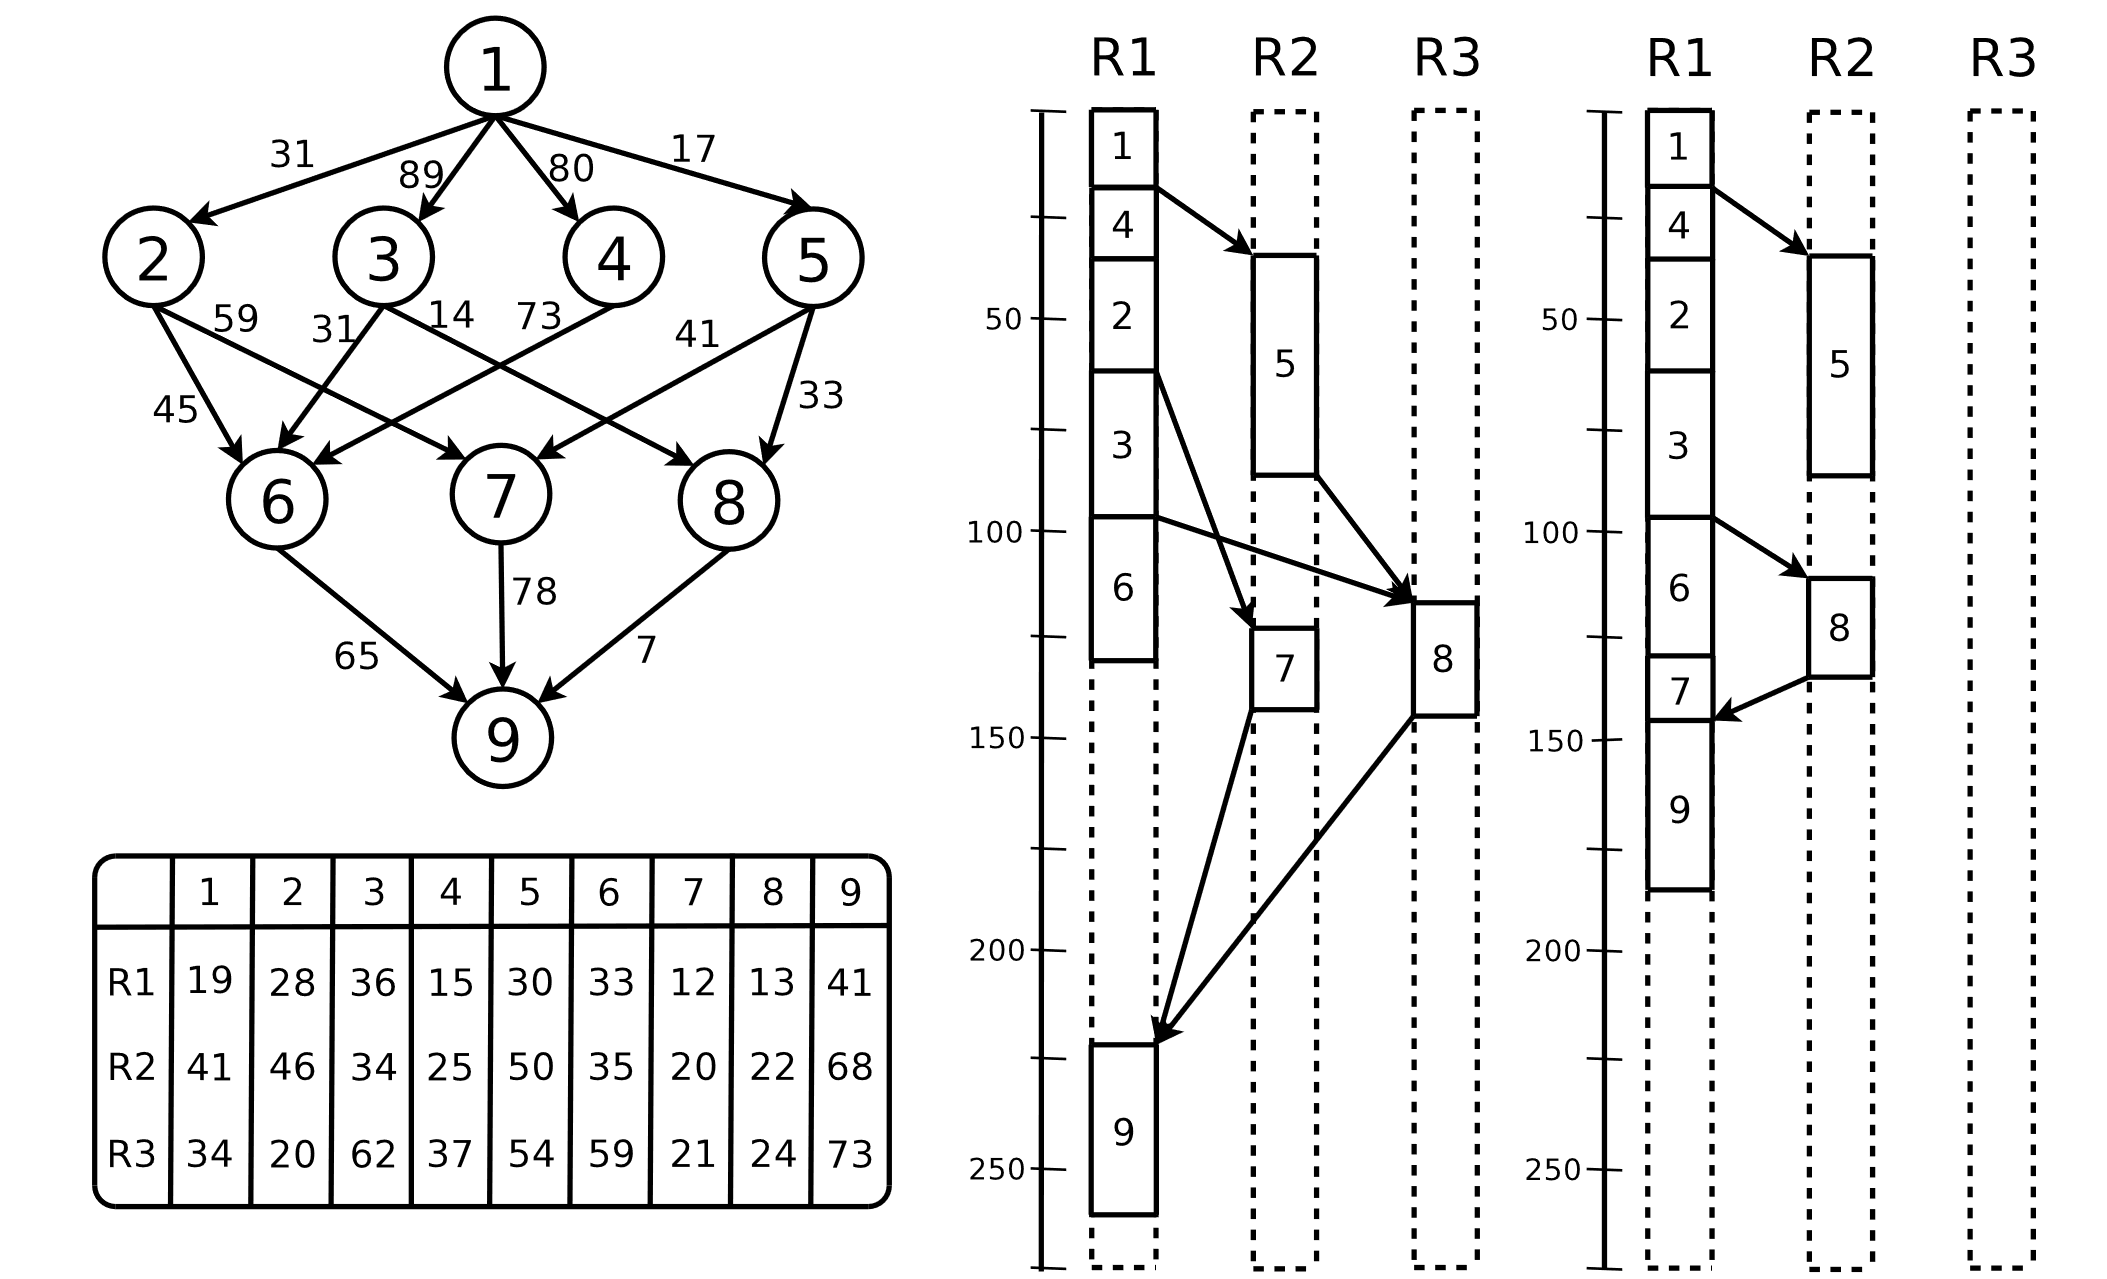
\includegraphics[width=0.85\textwidth]{heft_task_modeling}
        \bicaption{\quad 一种HEFT类算法\citep{topcuoglu_performance-effective_2002}对计算任务的建模}
        {\quad Modeling of heterogenous computing task by a HEFT like algorithm\citep{topcuoglu_performance-effective_2002}}
        \label{fig:heft_task_modeling}
    \end{figure}

    然而,因为该算法的贪心和短视特性,其性能在某些负载中离最优解相差很远,在之后的工作中,例如\citep{bittencourt_dag_2010},引入了有限的前瞻操作,使得在不增加太多时间复杂度的情况下让调度的最大完成时间相对于原算法平均约提升了20\%,之后的工作大多是为该算法添加其他的启发式步骤,如关键节点优先调度、悲观或乐观代价估计等等,但提升十分有限\citep{arabnejad_list_2014,zhou_list_2017}。
    
    HEFT类算法在最小的调度粒度是任务,这为该算法带来良好的可部署性的同时,也注定了在它的调度中不可能进行更细粒度的调度优化,从而最大限度地发挥硬件之间的并行性。因此总是存在着较多的空泡,甚至如图~\ref{fig:heft_task_modeling},会存在有些硬件从始至终都都维持着很低的利用率。且其算法偏向于将任务驻留在起始硬件节点上,对其他硬件利用率较低。

    \subsection{面向近存计算系统的调度技术研究与应用}
    
    由于架构和功耗的限制,PIM核心在局部性良好、计算密集型的负载运行时往往与CPU的性能存在着一定的差距,而CPU在运行局部性差、访存随机性高且不需要复杂运算的负载时,会面临很严重的访存瓶颈,此时PIM在总访存带宽上的优势会让其的性能远远强于CPU。然而,当任务调度不佳时,整个系统的能效比和性能会急剧下降,甚至出现负优化的现象\citep{gomez-luna_benchmarking_2021}。这也凸显了调度技术在近存计算系统实际应用上的重要性。也促生了一系列面向近存计算系统的调度技术研究。在相关调度技术研究中,不乏更细粒度的调度方法,此类研究通常会与近存计算系统自身特殊的体系结构设计紧密结合,同时涉及到对CPU硬件结构的修改,以完成更细粒度的调度优化,并期望利用硬件设计优化负载的调度和执行效率。
    
    在现有的工作中,针对近存计算系统,负载调度的思路大致分为两种:
    
    1. 从一致性入手:在尽可能少做数据搬移、保留近存计算带来的优势的情况下,通过在执行负载时维持数据块的一致性,从而做到CPU-PIM协同计算。一个典型的例子就是\citep{boroumand_lazypim_2017}中提出的惰性同步策略,该策略默认不使用同步,将不同任务地指令同时派发给CPU和PIM系统,使CPU和PIM乐观地共同执行涉及同一块存储的负载,并对TLB、页表结构和一致性协议进行定制,加入新的原子命令以处理完成工作的原子提交以及涉及脏数据块操作的原子回退机制,从而减少了内存总线中的通信总量。
    
    2. 从指令集扩展入手:通过扩展硬件,从而做到自动将访存密集型负载中的特定指令派发到至PIM系统中。一个典型的例子是工作\citep{ahn_pim-enabled_2015}里,在模拟器中对CPU硬件结构作出修改后,加入了局部性检测元件,并同时在CPU和PIM核心里扩展了新的、用于近存计算系统的特殊指令集。当运行时检测到局部性符合设定条件之后,CPU中特殊的控制器则会将特定指令派发到PIM元件上,以完成特定操作。通过这种依条件派发指令方式完成了CPU-PIM的协同计算。
    
    以上基于近存计算系统的负载调度策略,相对于~\ref{subsec:hetero_scheduling_intro}所描述的现实系统中的异构负载调度算法而言,其调度的单元从任务级细化到了指令级,可以在不改变编程模式的前提下完成更细粒度的CPU-PIM并行,但都涉及到对CPU和PIM内存本身硬件的修改,所以截至目前所有相关工作都是在模拟器中进行的,但是它们对该问题的解决思路,对基于实际DIMM近存计算系统负载调度框架的设计来说,仍具有很高的参考价值。

%%%%%%%%%%%%%%%%%%%%%%%%%%%%%%%%%%%%%%%%%%%%%%%%%%%%%%%%%%%%%%%%%%%%%%
\section{关键问题与研究目标}\label{sec:problems_and_goals}
    \subsection{存在的问题}\label{subsec:existed_problems}
    %访存密集型负载在真实计算任务中会与计算密集型交叉出现,任务判别问题
    %现实PIM系统与之前研究的模型不一致,实际应用时无法套用之前研究的成果去修改硬件
    %HEFT类算法粒度太粗,偏向于不去使用PIM系统
    %由于前几条,在现实PIM系统中,发挥其特殊架构优势时对调度的要求会额外的高
    本课题选用目前工具链与开发流程较为成熟的UPMEM商用近存计算系统作为实验平台,对该平台上负载的调度问题进行研究,由于其在近存计算领域被广泛使用并研究,具有一定的代表性,沿用~\ref{subsec:evolution_of_PNM}中的命名习惯,下文所述的“PIM计算系统”即专指“UPMEM商用近存计算系统”。
    
    在应用实际PIM计算系统时,尽管其特殊的体系结构在运行某些负载时提供了一系列引人注目的优势,其仍有若干关键问题亟待解决:
   
    首先,在负载方面,许多重要的计算负载都是访存密集与计算密集型任务混合的\citep{boroumand_lazypim_2017},此时只能依靠PIM和CPU进行协同才能获得最佳性能,然而对任务进行划分的方法、划分的粒度均是尚未被完美解决的问题。对于任务的分配以及CPU-PIM间通信策略的设计,会极大程度上影响整个系统的性能,甚至在许多情况下,依靠朴素地进行手动负载分配会导致显著的性能恶化,甚至是负优化(如图~\ref{fig:prim_benchmarks}中的NW、BFS等)。
    
    \begin{figure}[!htbp]
        \centering
        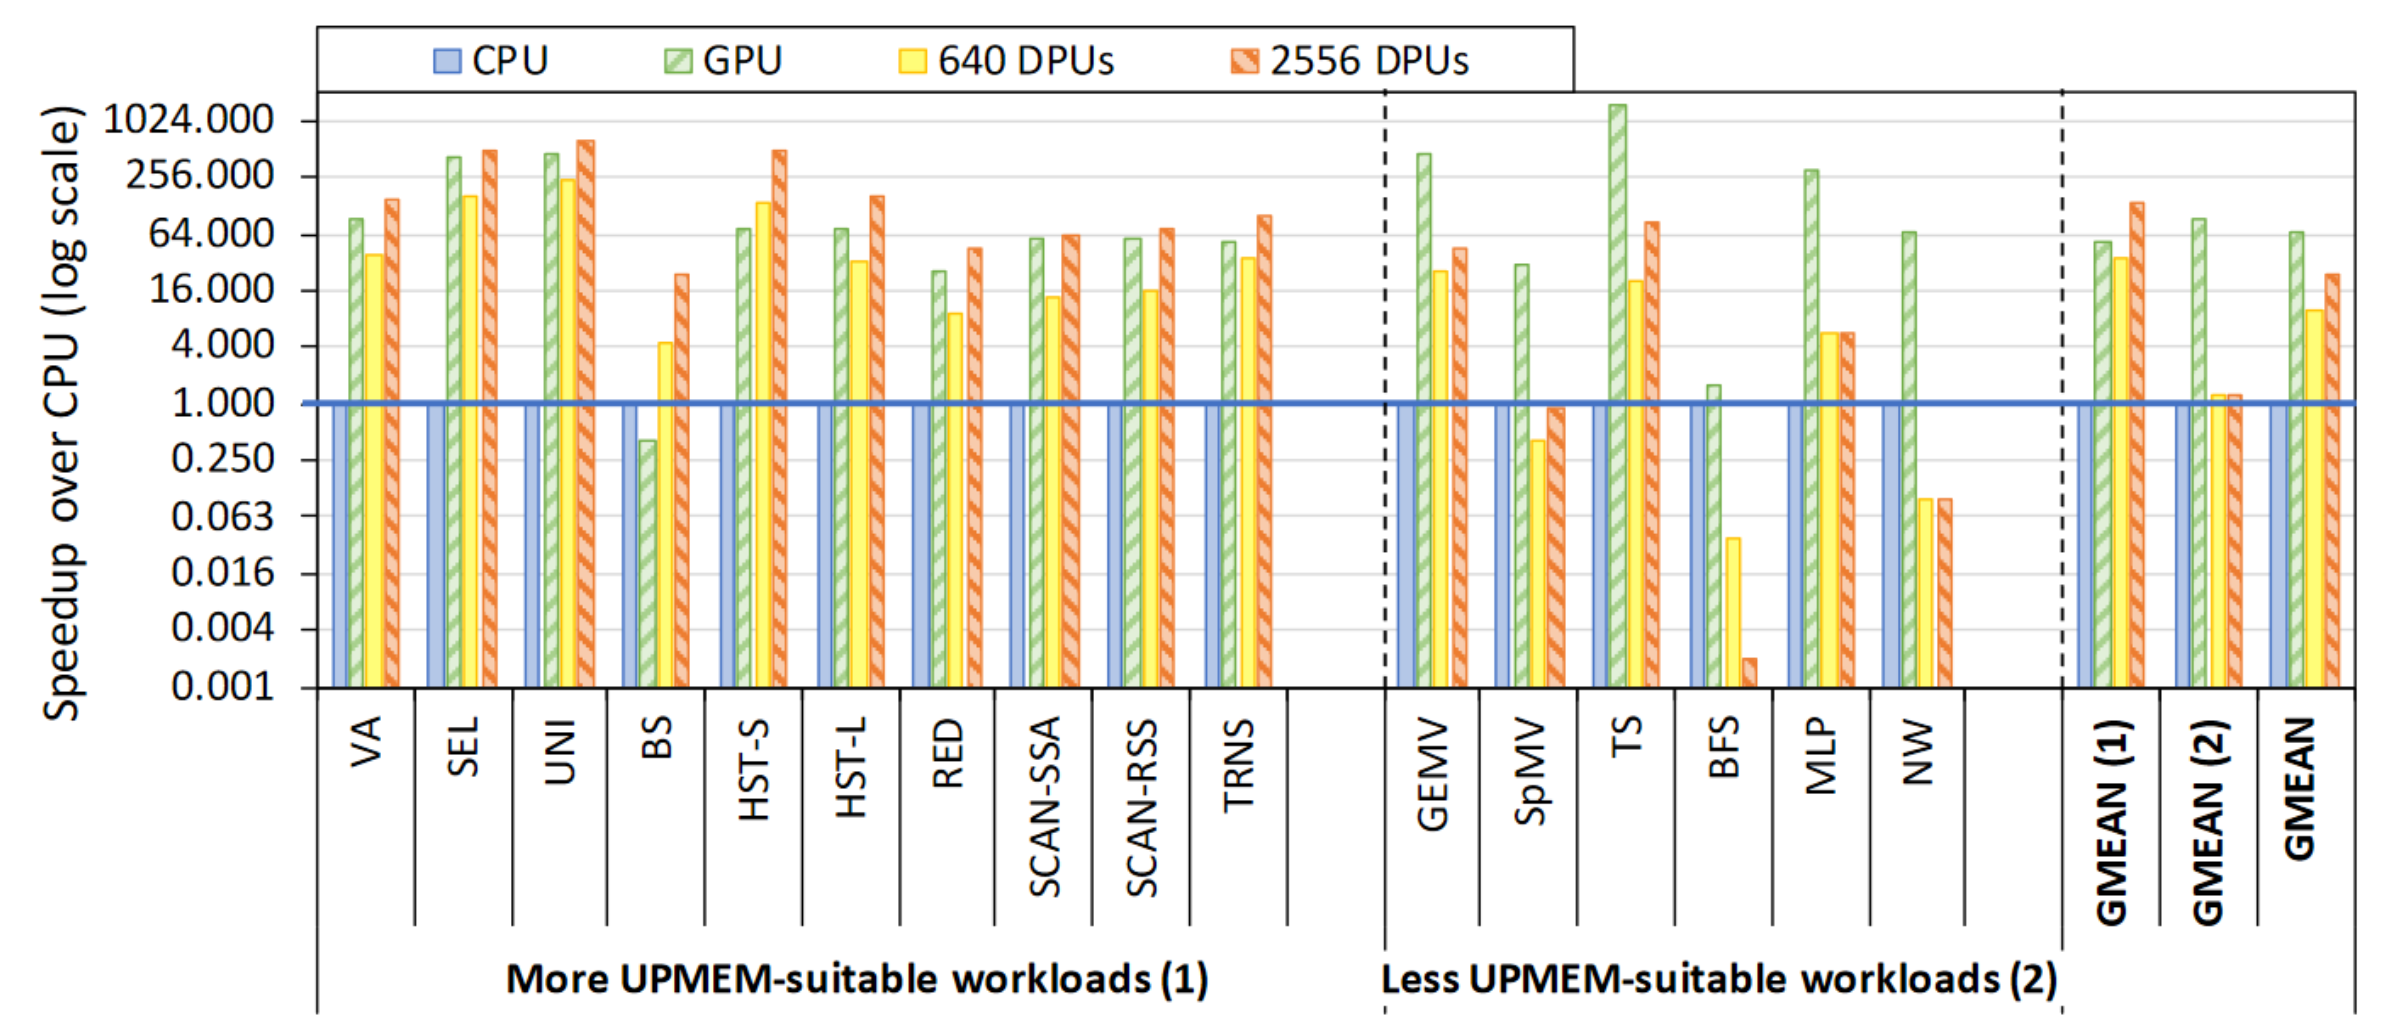
\includegraphics[width=0.85\textwidth]{prim-benchmarks}
        \bicaption{\quad 对基于DIMM的现实近存计算系统UPMEM的性能测试\citep{gomez-luna_benchmarking_2021}}
        {\quad Benchmarks of a real-world DIMM based PNM system, UPMEM\citep{gomez-luna_benchmarking_2021}}
        \label{fig:prim_benchmarks}
    \end{figure}
    
    其次,在硬件模型上,现实PIM计算系统的硬件结构与学术研究上所用的近存计算模型存在出入。本研究中所基于的PIM计算系统存在着若干个特征,显著区别于~\ref{subsec:evolution_of_PNM}中其他工作所基于的计算系统模型:
    
    \begin{enumerate}
        \item DRAM与PIM-MRAM非统一编址: UPMEM DIMM在使用中不与其他普通DIMM构成的主存储器统一编址寻址,获取其存储中的数据需要涉及到UPMEM-DIMM和主存储间的通信。
        \item PIM核间通信昂贵:UPMEM PIM核与核间不存在高速共享缓存和专用互联模块,所有PIM核间的通讯需要通过主存储器并由CPU直接介入,这会占用CPU资源以及访存带宽,带来很高的通信开销。
        \item 单个PIM-DPU只能直接进行小区间的PIM操作:单个UPMEM-DPU能通过DMA直接访问的空间只有64MiB,且区别于普通DIMM,UPMEM-DIMM在映射内存地址时不会将相邻的字节映射到不同颗粒上,而是会将8个相邻字节映射到同一个颗粒上的同一个DPU访存空间上。
        \item 近存计算内存不支持同时进行运算-传输:由于SDK底层将计算和传输抽象成同一类任务,并采用了任务队列的形式实现执行逻辑,UPMEM-DIMM无法在运行近存计算负载时处理与主存储器间的传输,以完成数据的预取和及时写回。
    \end{enumerate}

    此外,关于现有调度策略,目前主流的调度策略分为两种:或是基于贪心算法,依赖算法所调度的执行序,异步执行任务来完成任务间并行。又或是基于对CPU硬件结构本身的修改,依赖一致性协议或指令集扩展完成指令级并行,它们各自在优化任务分配、降低内存通信上取得了一定的成果,但是目前的方法在应用上的可行性和性能上仍次存在如下问题:
    \begin{enumerate}
        \item HEFT类算法无法使多器件协同处理一个任务,存在较多空泡;
        \item HEFT由于贪心策略,会导致短视,面对很高的通信代价,会偏向于自始至终将负载驻留在起始计算节点上。
        \item 基于一致性的调度策略对CPU做出结构性的修改,在现实系统中无法直接做到,且对于数据争用较为严重的负载,惰性同步会带来大量的回退开销。
        \item 基于指令集扩展的调度策略也对CPU结构进行了大量修改,且在复杂负载运行时,局部性判断器的决策质量会在很大程度上影响性能,造成较大开销。
    \end{enumerate}
    
    现有的工作或是因为执行逻辑不同、或是因为对硬件的改动,暂时无法直接应用于现实。
    
    最后,在执行逻辑上,以任务为粒度的调度框架所针对的负载模型和真实kernel的使用方式有着较大差异。而传统的函数级PIM kernel在使用时需要预先进行交叉编译,并在运行时传入UPMEM-DIMM中执行,这使得算子耦合性很强、灵活性较差,难以通过动态定制任务的执行逻辑和传输逻辑,以通过细粒度并行充分利用硬件资源。

    鉴于此,本工作将主要研究关于基于DIMM近存计算系统的调度技术,旨在结合现实近存计算系统,解决其在实际应用中存在的调度问题,从而更好地发挥近存计算体系结构在高性能计算领域的潜力。

    \subsection{研究目标}\label{subsec:research_goals}
    实际运行在近存计算系统的程序在处理任务卸载的过程中,一种朴素且被广泛使用的方法是依靠手动编程并管理管理负载的调度,将所有的负载分配和通信在程序编写时唯一确定。但这种“贪心式”的思路存在着弊端:当访存密集和计算密集型任务交替出现时,手动任务卸载中,过细粒度的同步或过粗粒度的任务划分,都会因频繁的数据搬移或过低的计算效率,从而带来不可忽视的性能开销,甚至会抵消近存计算带来的性能收益\citep{gomez-luna_benchmarking_2021,diab_high-throughput_2022}。一个可利用高层次任务信息进行调度,同时能结合硬件量化信息综合考虑到数据搬移开销、计算开销的调度策略是很有必要的。
    
    综合前文所述,当前近存计算系统存在着不同负载下性能差异大、运行负载时总体计算资源利用率低、CPU-PIM间数据搬移代价高等问题。且现有的异构调度算法在高代价数据搬移的前提下不能很好的利用计算资源,无法直接用于实际的近存计算系统的调度上。尽管现有的工作或是因为适用场景不同、或是因为对硬件的改动,暂时无法直接应用于现实。但它们仍存在着本文框架可以借鉴的思想:
    \begin{enumerate}
        \item 在任务内做到器件间的并行,应尽可能地消除异构器件闲等的情况,特别地,对于CPU-PIM这种双异构器件的系统,合适比例的负载划分所达成的器件间并行,会减少后续数据搬移所带来性能开销,从而起到预取作用。
        \item 基于贪心启发式算法对负载的调度会存在短视,从而形成局部最优解,在对于启发式的选择上,应尽可能采用更强的元启发算法以跳出局部最优。
        \item 基于局部性判断的调度方式,如PEI\citep{ahn_pim-enabled_2015},将局部性作为负载调度的唯一参考信息,但忽略了实际近存计算核心处理能力与CPU间的不匹配,且无法参考后续的任务信息以完成更大范围的调度,从根本上来说仍是短视且追求局部最优的。应利用高层次的任务信息从而尽可能避免短视决策所带来的性能损失。 
    \end{enumerate}
    
    为解决这些问题,本课题旨在基于实际的近存计算系统,研究并设计一种高性能、细粒度的调度方法,以实现对混合负载的细粒度任务划分和调度优化,从而得到相比于原有调度方法更高的性能与能效比。
    
    
    本课题的研究目标及设计可总结为以下三个要点:

    \textbf{混合负载类设计}
    
        目标:解决近存计算系统不同负载下性能差异大的问题。
        
        设计: 提出一种可细分、适用于CPU与PIM协同计算的异构负载类设计,通过算子层面的跨平台接口,实现任务分配与计算协同,为后续的模块设计建立基础。

    \textbf{基于混合负载类的协同计算框架设计}
    
        目标:提高运行负载时总体计算资源利用率。
        
        设计:基于混合负载类,设计调度策略生成模块。用先验知识进行任务分配的分治方法,包括量化器、回归拟合模块、策略价值判别模块及元启发策略优化器,以确定所有算子在不同器件上的任务分配比例,从而优化整体性能。

    \textbf{调度策略生成器与优化器设计}
        
        目标:降低负载间数据搬移代价,提高计算效率。
        
        设计:基于负载类的可分性,设计异步执行模块。利用细粒度异步并发执行缓解高传输代价带来的同步开销。并使用懒惰写回策略,最大限度地减少器件间传输空泡以及数据搬移开销,提高CPU-PIM系统整体的计算能力。
    
%%%%%%%%%%%%%%%%%%%%%%%%%%%%%%%%%%%%%%%%%%%%%%%%%%%%%%%%%%%%%%%%%%%%%%
\section{本文的贡献}\label{sec:contributions}
针对近存计算系统在实际应用时所面临的性能问题,本文提出了一系列创新性的解决方案。本文所涉及的贡献主要体现在以下几个方面:

\textbf{基于算子的负载抽象与跨平台算子基类的构建}

本文采用了一种以算子为核心的负载表达方式,并在此基础上设计并实现了一种新型的跨平台算子基类。这种基类不仅继承了算子表达方式的高内聚低耦合特性,便于编程实践和并行调度,而且通过重构UPMEM原有的工具链匹配了跨平台算子,增强了算子在不同计算环境中的适应性和可重用性。此外,该基类支持按比例调控不同计算单元的任务量,有效减少了因不当任务分配而引起的性能损耗,提升了负载执行的灵活性和效率。 通过这一综合性的贡献,本文在近存计算系统中实现了单一负载多设备执行的方法,还为异构计算环境中的算子设计与实现提供了一种新的范式,这对减少异构设备通信、提升计算任务的执行效率和系统的整体效能产生了积极影响。

\textbf{调度策略生成及优化模块}

本文基于混合负载类设计了一种新的调度策略生成及优化模块,用于生成并优化CPU-PIM间任务的调度。这种方法是一种基于先验知识的分治方法,能够有效提高计算资源的利用率。 具体到策略生成模块的构成,本文的贡献包括: 

	运行时性能量化器:本文开发了一个量化器,用于在预热阶段收集算子计算和传输的性能量化数据,为后续模块提供必要的性能数据。
 
	量化性能拟合模块:本文实现了一个回归拟合模块,用于建立和训练可泛化的性能模型,用于调度价值评估。 
 
	调度价值判别模块:本文设计了一个调度价值判别模块,可基于量化拟合数据用于评估调度策略的价值,并为优化器提供反馈。
 
        元启发调度优化器:本文复现并采用了若干元启发优化算法,用于在有限时间内搜索最优调度策略,以提高系统的性能与能耗比。
        
 总结来说,本文为现实基于DIMM近存计算系统执行混合负载时的性能优化提供了一种新型解决方案。通过以算子中心的负载表达、跨平台算子基类的设计以及基于元启发算法的调度优化器的设计,本文不仅解决了性能差异、数据搬移代价高和计算资源利用率低的问题,还提高了系统的计算性能与能效比,有望为推进基于DIMM的近存计算这一技术的实际应用做出一定贡献。
%%%%%%%%%%%%%%%%%%%%%%%%%%%%%%%%%%%%%%%%%%%%%%%%%%%%%%%%%%%%%%%%%%%%%%
\section{本文的组织}\label{sec:doc_organization}
第一章概述课题的研究背景与意义。
从存算单元性能发展所形成的“剪刀差”和存储墙现象入手,
介绍近存计算技术的研究背景,及其从设计理念到现实商业落地的发展历史,简要介绍了不同近存计算技术的设计思路和系统结构。
随后简要讲述了近存计算技术在应用时所面临的挑战,并阐述异构调度算法与本课题涉及研究内容的联系。
接着介绍了本文所涉及到的领域在国内外的研究现状,结合目前的主流方法引出研究中的
关键问题和研究目标。最后介绍了本文的贡献和组织结构。

第二章介绍了本课题所对应项目中涉及到的相关理论和技术。
首先,以粒度由粗到细的方式,依次介绍了目前主流的异构调度算法,以及面向PIM系统的细粒度调度方法。
随后介绍了本课题所设计的调度算法中所采用的的元启发优化算法。

第三章首先介绍了基于SKMD的负载执行时的基本流程。
随后结合UPMEM近存计算系统的负载执行流程以及常见性能瓶颈的归纳,
引出本课题对UPMEM-SKMD类型可分混合负载类的建模与设计,以及基于该负载建模的工具链重构。
随后介绍了该负载建模下的计算图执行逻辑的设计与实现,
同样以粒度从粗到细的顺序,依次介绍计算图执行逻辑中:算子间调度逻辑、算子间传输逻辑以及算子内计算逻辑的设计与实现,
并在最后对本章所设计并实现的基于SKMD的CPU-PIM协同计算框架进行总结

第四章主要介绍负载划分及调度优化算法的设计与实现。
由于本课题中的负载划分和调度优化会涉及到性能量化模型和元启发优化算法,
本章先从性能量化模型的训练流程和元启发参数优化的基本流程入手,
分别展开基于UPMEM的性能量化回归学习模块,以及面向负载量化回归学习模型的元启发调度优化模块的具体设计与实现
最后总结本章所介绍的负载划分及调度优化算法,
并对整个基于DIMM近存计算系统的调度优化方法进行系统讲解。

第五章主要介绍了本课题的实验结果和分析。
本章分为实验验证、验证结果和数据分析三段内容
首先介绍了测试数据集,分别介绍了测试中使用的不同计算特性的算子、不同拓扑结构的计算图
以及随机负载生成算法以及其最终生成的、用于本次测试的混合负载集合。
随后介绍了实验对结果的评价指标。
在验证结果部分,分别展示了算子性能量化回归模型的回归结果,不同负载中元启发调度优化算法的收敛情况,
以及经不同调度策略调度后,各个实验负载整体的性能和能耗情况。
在数据分析部分,分别对本课题所提出的调度算法进行优化效率、稳定性的分析,以及对调度结果进行进一步评估。

第六章则是对全文的总结,并提出未来可以继续研究与改进的方向。

\chapter{相关理论与技术}\label{chap:Theory_And_Techs}

\section{基于DIMM的近存计算技术}\label{sec:PNM_DIMM_intro}
    \subsection{体系结构特点}\label{subsec:arch_talent_intro}
    基于DIMM的近存计算是一种旨在缓解处理器与内存间数据传输瓶颈的计算范式。该范式的体系结构特点可以从以下几个方面进行阐述:

    \textbf{以数据为中心的设计理念}:该体系结构强调以数据中心的设计理念,即将计算任务尽可能地移至数据所在位置执行,以此减少数据移动带来的开销。这种设计理念有助于提升大数据处理和分析任务的效率。
    
    \textbf{内存与计算单元的紧密集成}:该体系结构的核心特点是将计算单元(如处理器核心或加速器)与内存阵列紧密集成在一起。这种设计可以减少数据在处理器和内存之间的移动,从而降低延迟并提高能效。
    
    \textbf{基于成熟的DIMM主存储技术}:该体系结构选择被广泛应用于普通计算机系统中的DIMM主存储技术作为基石,通过将计算能力下放至DIMM周围,并改变CPU与其之间的交互逻辑来实现近存计算,普遍对原有计算机体系结构的修改较小,有利于开发和实际部署。
    
    \subsection{UPMEM近存计算系统结构}\label{subsec:UPMEM_arch_intro}
        \subsubsection{硬件体系结构}\label{subsubsec:UPMEM_hardware_arch}
        图1-1是近存计算系统UPMEM的结构示意图,该系统是截至本文书写时(2023年10月)市面上唯一使用存内计算架构的商用计算系统,也是本文所有实验所基于的硬件系统。
        
        UPMEM在传统DIMM内存中的每一个64MB颗粒上都集成了一颗低功耗的、基于RISC-V架构的通用处理核心, 以及64KB的高速工作内存(Working Memory) 和24KB的指令内存(Instruction Memory)。该核心拥有14级流水线,其中有3级可同时完成,在实际计算中采用小任务块(tasklet)的实现方式来完成细粒度的计算划分,用于充分利用流水线的资源,其最优大小根据运行时计算队列的组成结构而定。对于该处理器的设计架构,一般来说大于11的tasklet数才能充分利用流水线[10]。
        
        UPMEM-PIM计算系统其实更类似于一个不需要考虑节点宕机(稳定性高)、通过主存储器通信(不涉及网络通信)、不用考虑拜占庭故障(可靠性高)的分布式计算系统\citep{chen_simplepim_2023}。频繁的PIM核间通信所带来的开销,会很大程度上抵消其架构在访存延迟和功耗上带来的优势。如果希望最大限度地发挥该架构的优势,则需要在算子层面尽可能地利用PIM处理器的并行性,避免核心间的频繁通信\citep{gomez-luna_benchmarking_2021}。因此,运行于PIM系统的程序在编写时往往需要与实际硬件结构紧密结合、审慎处理所有的数据传输操作。这给PIM系统的编程和调优带来了额外的复杂度\citep{chen_simplepim_2023}。
        
        一个典型的UPMEM PIM系统中包含20条8GB的PIM-DIMM,其中每一个PIM-DIMM包含128个低功耗DPU,整个系统共集成了2560个DPU,对应合计160GB大小的存内计算空间。它们与4条64GB的普通DDR4-DIMM内存各自共享两条内存通道。

        \subsection{工具链与开发环境}\label{subsubsec:UPMEM_toolchain_arch}

        \subsection{软件模型和编程接口}\label{subsubsec:UPMEM_software_model_and_interface}
\section{异构计算系统调度技术概述}\label{sec:brief_intro_of_heterogenous_scheduling}
    \subsection{基于表的负载调度算法}\label{subsec:list_schedule_algorithm_intro}
    %HEFT like
    \subsection{采用启发式学习的负载调度算法}\label{subsec:heuristic_based_scheduling_intro}
    %HEFT-with-heuristics 
    \subsection{单一负载多器件执行(SKMD)调度技术}\label{subsec:SKMD_intro}
    %SKMD
    \subsection{应用于PIM系统中的细粒度调度技术}\label{subsec:fine_grained_PIM_schedule_intro}
    %LazyPIM, PEI

\section{基于元启发的参数优化算法}\label{subsec:metaheuristic_based_args_optimization_intro}
    \subsection{粒子群算法}\label{subsec:PSO_algorithm}
    \subsection{算术优化算法}\label{subsec:AOA_algorithm}
    \subsection{爬行生物优化算法}\label{subsec:RSA_algorithm}

\section{本章小结}\label{sec:chap2_summary}
本章首先对基于DIMM的近存计算体系结构的特点进行了简要的介绍,随后详细介绍了本文所基于的现实近存计算平台UPMEM的系统结构,包括硬件体系结构、工具链和软件模型及编程接口。接着,结合~\ref{subsec:existed_problems}节所提到的现有问题与UPMEM平台的特性,介绍了类似的异构计算系统调度技术,包括基于表的负载调度算法、采用启发式学习的负载调度算法、单一负载多器件执行技术以及专门应用与PIM系统中的一些细粒度调度技术。最后对本课题中被复现并使用的元启发参数优化算法(见~\ref{sec:metaheuristic_optimizer_facing_SKMD_regression_model}节)进行了介绍。

\chapter{研究方法与过程}\label{chap:Method_And_Research_Procedures} 

\section{研究方法}\label{sec:research_method}
  %方法部分,讲述“切分+按比例派发+同时运行”形而上学的方法论、以及其成功的理论依据
  %--------------- 此部分采用“分总”结构叙事 -------------
  \subsection{对UPMEM系统实际运行时性能瓶颈的归纳}
  \subsection{具有可分性的跨平台负载类设计}\label{subsec:dividable_load_abstraction_design}
  针对近存计算核心在执行不同计算任务时性能差异大的问题,本课题综合以往异构计算的最佳实践,选用以算子为中心的负载表达方式,并重新设计了算子的封装形式,设计并实现了一种便于协同计算的跨平台算子基类,从而为算子提供跨平台、按比例调控不同部件所执行的任务量的能力,从而减轻了传统算子将任务完全错误分配到不合适的器件上以致产生负优化的可能。

  由于使用算子所表达的计算任务高内聚低耦合,易于书写、维护和重用,且便于并行执行和调度,在工业界异构计算框架[41], [42]里正被广泛地采用,是一种被广泛验证的设计。单个算子作为一类具有相似计算特征的负载的共同抽象,可以被看作是一种输入向量到输出向量的映射。

  然而,目前常用的算子在设计、优化和最终封装时往往针对的只是单一硬件后端,这就导致了:1. 算子作为负载的抽象,在设计时却并未考虑到多个异构计算器件的协同工作,转而只能使其依赖于上层逻辑中对异构设备中同一算子的分配和调用,这就在上层逻辑中增加了在算子调用、负载分配上的复杂度。2.为了达到多器件协同,需要手动管理任务分配的比例以及器件间的同步,这与算子的设计初衷相违背。3. 涉及到多个复杂算子时,通过手动管理负载分配来充分发挥异构执行单元各自的优势,获得最优的性能十分困难。众多因素阻碍了在算子层面上异构计算器件的协同,从而导致了负载运行时异构器件的闲等和低利用率。

  因此,本课题提出了一种可细分、同时可用于PIM和CPU的异构负载类设计。相似的设计如PEI[23]中,作者将近存计算算子与CPU指令一一对应并用硬件根据局部性决定指令派发,而在SKMD[43]中,作者使用OpenCL书写算子并分别编译CPU和GPU程序。考虑到UPMEM系统尚未存在对OpenCL的支持、且修改CPU硬件结构是不可行的,本课题借鉴两种设计中的长处,并针对本课题所基于的现实近存计算系统,设计了一种适用于CPU与PIM协同计算的、可按照指定比例进行任务划分的负载类,能够在不修改原有算子书写模式的同时,便于CPU-PIM协同计算时的任务分配与任务间调度,进一步提升运行效率。

  \subsection{调度策略生成模块设计}\label{subsec:scheduleGen_module_design}
  针对运行负载时总体计算资源利用率低的问题,本课题基于3.2.1中设计的混合负载类,设计了一种生成并优化CPU-PIM间任务分配比例的调度策略生成模块,以确定所有算子在不同器件上的任务分配比例,本质上是一种利用先验知识进行任务分配的分治方法。

  策略生成模块由量化器、回归拟合模块、策略价值判别模块及元启发策略优化器组成。其中:

  1. 量化器用于在预热阶段收集算子在不同参数下的运行性能量化数据,并提供给回归拟合模块用于建立量化数据的一个回归模型。

  2. 回归拟合模块用于接收量化器提供的数据,并根据其不同的参数进行回归拟合,并获得训练好的性能模型,本质上是一个通用的统计学习回归模型 

  3. 策略价值判别模块的核心是由一组涉及到传输、计算的时间及能耗的方程所构成的损失函数。该模块接收优化器所提议的调度策略,并传递给回归拟合模块来获取预测的量化信息,使用该信息以评估被提议策略的价值,最终将策略的价值评估提供给元启发策略优化器,以及(可选的)输出该策略在运行中预计情况下的量化信息,如时间和能耗。

  4. 元启发策略优化器负责与策略价值判别函数交互,并在达到终止条件前为回归拟合模块提供新的策略提议,本质上是一个通用的元启发优化算法,参数空间的维度等于算子的数量,参数范围为0到1的闭区间(有一些算子如load-store只能由CPU执行)。

  这四个模块中,量化器作为直接与负载进行交互的模块,会对每一个算子在不同参数下的性能数据进行尽可能详尽的测量,其对量化数据收集的完备性会影响使用该数据进行训练的回归拟合模块的拟合准确性,相对应地,在回归拟合模块中,对于合适回归算法的选用,会影响到最终训练出的回归模型的泛化性,而泛化性越好的模型在推理时得到的预期量化数据就会越贴近真实数据,使价值的判别更加具有参考意义。价值判别模块作为整个策略生成模块的核心,会根据预测的量化信息对该策略的价值做出评定,其中的价值函数的设计需要充分考虑对负载调优的偏好(性能或能耗),一个好的价值函数会使元启发优化算法更容易收敛并提供一个指标符合期望的调度策略。而元启发策略优化器作为对整个优化空间的一个搜索器,其收敛速度,搜索能力以及逃离局部最优解的能力都会影响整个调优过程的性能,并决定最后策略的优劣。

  \subsection{整体执行逻辑设计}\label{subsec:overall_logic_design}
  (需大改)
  针对负载间数据搬移代价高的问题,本课题采用了经典的计算掩盖传输的思路,但考虑到现实PIM系统中MRAM和DRAM非统一编址、且两者间传输带宽不高,为了进一步提高系统的计算效率并降低空泡,本课题利用3.2.1所设计的负载模块的可分性,将切分后的算子的每一个部分视作一个异步任务,该任务将在按照调度策略进行传输后,立即异步执行以及(按策略决定是否)写回,以细粒度划分任务的形式避免了传输时的同步停等,并提升传输总线在整个执行时间上的占空比,避免总线拥挤。

  将按比例划分后的任务按照依赖关系,以生产者-消费者模型进行派发,每个器件处理不同比例的任务,通过该异步执行模块推进任务进展、避免频繁同步和通信,以这种设计模式极大地减少了器件间闲等空泡,最大的利用了CPU-PIM的计算能力。

\section{研究过程与具体实现}\label{sec:research_procedure_and_implements}
  %过程部分,讲述其实现与伪代码
  %--------------- 此部分采用“总分”结构叙事 -------------
  \subsection{混合负载类建模与基于建模的工具链重构}\label{subsec:load_abstraction_and_toolchain_refractor_impl}
    \subsubsection{混合负载类建模}\label{subsubsec:load_abstraction}
    解决负载调度问题,首先要涉及到对负载本身的建模,也要同时考虑到运行负载的系统:

    在UPMEM PIM系统运行近存计算负载的关键步骤是PIM程序的交叉编译和PIM-MRAM 到DRAM间数据流的控制。以简单的向量加(Vector-Add,VA)算法为例,典型的执行流程是:1.交叉编译运行在PIM核心上的代码2.使用UPMEM API分配若干个可用的PIM DPU 3.在CPU部分的代码中为PIM kernel开辟输入输出缓冲区 4.将交叉编译后的代码载入PIM核心 5.传输参数和缓冲区数据到指定的核心 6.启动PIM端代码的执行 7.同步等待执行完毕并传回数据至主存储区的输出缓冲区。

    在仅执行单一kernel或若干个无数据依赖的kernel时,该流程可以很好的完成任务,但多阶段任务中,由于现实中PIM-MRAM和DRAM并不统一编址,对PIM在不同kernel间MRAM上下文的保存和使用就成为了减少MRAM-DRAM通信的关键,然而在被广泛使用的流程中,kernel本身由于提前被静态编译为二进制文件并载入,是无法利用运行时的调度信息(原地使用上下文继续计算或清理堆内存、等待CPU传输后计算)和可变参数(缓冲区大小等)的,这不利于负载在有上下文情况下的驻留或调度。

    故在实现适用于负载调度系统的抽象负载类时,本课题的设计如下:

    考虑到PIM元件间通信需要经过主存,无直接互联、通信开销大,本设计中所有的算子的书写都必须满足可分的前提,可以拆分为若干个任务块,且对应特定的、无重叠的输入输出数据块。

    考虑到PIM元件访存延迟比CPU低,但从CPU端访问PIM核心需要通过内存通信(非统一编址,访问开销大),所有负载对象在设计时会同时包含PIM kernel和 CPU kernel,分别用于执行驻留PIM上的代码,以及在CPU上执行相同功能的代码。

    考虑到使用PIM核心时需要预先编译其二进制,并在调用kernel前传入PIM元件,难以动态定制任务执行的逻辑。本设计中所有PIM kernel在调度策略决定后在宿主机调度协程中进行传参并编译,所有同一任务下切分的负载对象共享相同的二进制。

    至此,如图一个可以将任务划分为若干个负载块的负载抽象就建立完毕了,该负载类同时包含可以在CPU和PIM上执行的kernel,以及控制其具体执行逻辑的上层控制函数(control wrapper function),其中上层控制函数和调度器类是友元关系,可以根据调度器的决策来进行数据传输后执行、原地执行或上下文执行,从而在指定的硬件执行对应的算法。
    
    \subsubsection{基于负载建模的工具链重构}\label{subsubsec:toolchain_refractor}
    由于UPMEM-PIM DPU(以下简称为DPU)和通用处理器的体系结构不同,实际运行在DPU上的二进制程序将使用被特殊定制的C标准库和自定义原语,故所有DPU的程序都需要在UPMEM提供的、基于CLANG-LLVM框架开发的特殊C编译器中进行编译。而宿主端的程序可由普通的C、C++、Python或JAVA书写并使用通用编译器/解释器进行编译或解释运行。通过直接或间接地调用C API中的函数,宿主机端程序可以在运行时用指定编译好的DPU二进制文件绝对路径的方式,将由特定编译器编译好的DPU二进制代码动态加载到指定的DPU上,并控制数据的传输以及DPU程序的执行,而有关于算子数据类型、DMA参数等与宿主机公用的信息也都在编译时确定并再也无法进行变动,更无法在运行时进行调优。

    在编译构建整个项目的时候,一种常用的做法就是书写一个特定的Makefile并手动管理依赖关系,将DPU和宿主机代码通过规则中调用shell命令的方式控制编译参数与二进制文件存放位置。该方法本质上是书写一个复杂一些的脚本。这种分离编译并传入二进制绝对路径执行的做法,自Prim-benchmarks之后,在众多基于该系统的项目中都在沿用,虽说在操作上和理解上难度不大,但是在应对多算子、多数据类型甚至是运行时泛型算子的情况时会十分繁琐,而这些情况在调度框架中是十分常见的,故本课题在该方面做了以下的工作:
    
    (a). 用C/C++同时兼容的语法书写Consensus.h头文件,在其中包含对数据类型标识、公用结构体等的宏定义,最大限度减少编译期固定的参数定义,而将可以在运行时确定的参数以结构体的形式传入DPU,保留灵活性

    (b). 受tag\_invoke[44]的启发,在Consensus.h中,使用宏编程在C语言中仿照实现了高级语言里的类型反射行为,通过在宿主机和DPU间通过共有的类型标识传递类型信息,使得DPU可以在硬件支持的十余种数据类型、以及Consensus.h中声明的复合类型范围内支持泛型算子的执行,其结构大致如图1所示。

    (c). 采用现代化的CMake构建系统构建整个项目,为项目的混合编译编写了特殊的CMakeLists,自动管理宿主机和DPU程序的编译方式以及二进制文件路径,并暂时使用C++17标准的filesystem库进行运行时路径解析,避免使用绝对路径索引DPU二进制文件,提升鲁棒性,该项目目前的目录树如图2所示。当前正在进行的工作中还包括宿主机代码编译期DPU二进制文件嵌入行为的编写,在该项工作完成之后,Release版本的近存计算程序中宿主机和DPU端代码由路径索引的二进制依赖关系将不复存在,将更有利于程序的移动和部署。

    考虑到整体性能和开发效率,本课题选用现代C++语言作为宿主机编程语言,这就意味着需要和宿主机C++开发库进行交互。

    UPMEM官方所提供的通信、执行库的编写语言和原生接口都是以C的形式提供的,官方提供的其余语言API,如C++、Python、JAVA接口都是由C语言接口进一步封装而得来,本课题需要使用的C++ API在实际使用中暴露了多个问题:

    (a). 健壮性问题(数据类型越界、内存泄漏)

    (b). 继承关系混乱(不规范的派生关系)

    (c). 成员函数重载过多且封装不良,不利于分析

    综上,本课题弃用原始的UPMEM C++ API并重新封装原生的C接口,目前已将原来作为类成员的通信方法分离并重构完毕,构造成单独的、可量化的算子并继承自统一的算子基类(如图3),同时在基类中引入全局的ChronoTrigger指针(见工作3),使一切有关于计算和传输的行为都可以被统一调度和量化。

  \subsection{调度策略生成与优化模块实现}\label{subsubsec:scheduleGen_module_impl}
    \subsubsection{运行时量化模块ChronoTrigger的设计与实现}\label{subsubsec:ChronoTrigger_impl}
    该量化器的底层通过Intel PCM直接在运行时读取系统硬件性能计数器,从而获取暂态或一段时间内的性能信息,本实现将其抽象为一个单例模式的“探针管理器”,通过tick-tock(如4-6)的方式对程序中某一部分进行量化数据的采集,并使用哈希表的方式将测试时手动传入的程序段名称映射到指定的Report数据结构中,该结构里包含着若干种性能量化指标的统计量。

    在复杂度和精确性上,ChronoTrigger对性能指标统计量的计算(如均值、方差)都是增量式的,不需要遍历并存储历史性能数据,在时间和空间上的开销均为常数量级,便于后期动态调度时对统计量的即时分析,且本量化器会在构造时进行100次的tick-tock空转并生成一个\_\_BIAS\_\_报告项,用于在输出时纠正其他报告中存在的系统偏差。
    \subsubsection{性能量化数据回归模块的实现}\label{subsubsec:perfRegressor_impl}
    \subsubsection{策略评估及元启发策略优化模块的实现}\label{subsubsec:eval_optimizer_impl}
    由于本课题涉及到高维空间内复杂函数的最优解寻找,且对其的直接求解是NP完全问题,故采用元启发优化算法对全局最优解进行逼近。

    截至目前,本工作已复现了3种元启发算法,分别为同、异步的粒子群算法[45](Particle Swarm Optimization, PSO),算术优化算法[46](Arithmetic Optimization Algorithm,AOA)和爬行优化算法[47](Reptile Search Algorihm, RSA),并以C++泛型类的形式将其书写完毕,在实现中使用泛型函数指针,将目标函数的定义与优化器分离,可以对自定义决策质量判别函数进行最优解的求取。在验证后,于若干个高维、多局部最优点的函数优化中取得了与原论文中接近的效果,并获得了较好的性能。现已将该三种算法封装完毕并设计继承了统一的优化器接口以供主项目调用

  \subsection{策略执行逻辑实现}\label{subsec:overall_logic_impl}
  由于课题将近存计算系统看作是一种特殊的异构计算设备,且该设备和CPU间的阻塞传输对整体性能的影响较为严重,所以在合理划分负载分配比例的工作上,要想进一步提升整个调度系统的性能,一个异步的传输-执行模块对于提升该系统的性能是十分重要的。经过试错与总结,本课题最终选用未来将引入至C++26标准库的stdexec提议(P2300),以结构化异步并发(Structured Asynchronous Concurrency)的设计思路来构建整个异步传输-执行模块。

  在结构化并发的设计思路里,所有的异步计算主要由四种概念所支撑,其关系可见图4-8:

  Sender(或译为发送者):是对于异步计算工作的描述,可以被认为是计算图中的一个计算节点,会包含一个用于连接Receiver的方法,用于和自己工作对应的接收者建立联系。

  Receiver(或译为接收者):是对传统异步计算中“回调(Callback)”的一种抽象,具有三种接受发送者信息的方法,分别用于接受异步工作的正常返回值、错误信息或提前终止信号中的一种。

  Operation\_state(或译为工作状态):是真正存储工作上下文的一个类,具有启动异步任务的能力,与每一对Sender-Receiver都是一一对应的。

  Scheduler(或译为调度器):调度器是一个轻量级句柄,代表一种将工作调度到执行资源的策略。调度器概念由一个单一的、返回Sender的方法定义,这个返回的Sender将使依赖于该Sender的后续有任务调度在由调度器确定的执行资源上完成。

  本课题在抽象负载类的设计(见3.2.1)中,考虑到传输同步的开销,要求所有任务都是可以切分成若干个子任务并进行拼接完成计算,而在P2300中,所有异步执行的任务都被建模为一个Sender(发送者),而Sender可由若干个Sender所构成,在结构上是自相似的,在这一点上与本设计匹配,可以用较少的额外工作进行负载类的重构。

  在实现中,所有Sender所表示的工作都被定义是懒惰(lazy)的,在没有显式执行同步获取以最终结果前,所有的异步执行任务的声明,都只是在建立依赖关系以及构建回调链条。再加上Sender的底层实现是通过模板嵌套的形式,大多数Sender算法本身就具有可分和可组合性,编译器能够看到使用Sender描述的一系列工作形成了一棵尾调用树,从而实现了内联化并消除了大部分内部机制所带来的开销。所以它们具有在编译时期利用编译器将多个算子融合在一起并形成Sender链的机会,进而结合可分的算子构造,完成多个算子的自动融合。

  本课题完成了基于P2300的Sender-Receiver进行了线程池性能测试实验,在未来的补充实验里,会使用Sender-Receiver模式对整个执行流程进行异步化加速。

  至此对本课题所设计的调度逻辑的叙述就已经完成了,关于运行本调度算法的一个典型示例以及伪代码如图 4 9:
  

\section{本章小结}\label{sec:chap3_summary}
\chapter{实验验证与结果分析}\label{chap:Result_And_Analysis} 
\section{实验验证}\label{sec:validation}
  实验部分,讲述benchmark的选取以及测试标准
  \subsection{数据集}\label{subsec:dataset}
    \subsubsection{算子集合}\label{subsec:operator_set}
    \subsubsection{计算图集合}\label{subsec:compute_graph_set}
  \subsection{实验评价指标}\label{sec:evaluation_metrics}
\section{数据分析}\label{sec:result_analysis}
\section{本章小结}\label{sec:RAA_summary}


\chapter{总结与展望}\label{chap:Summary} 

\section{本文工作总结}\label{sec:result_analysis}
\section{下一步研究方向}\label{sec:TODOs}

%---------------------------------------------------------------------------%
% main content

%-
%-> ----------- 后文 -----------------
%-> Backmatter: 参考文献、附录与致谢获奖
%-
\backmatter
% ---- 参考文献 ----
\intotoc*{\cleardoublepage}{\bibname}% add link to toc
\artxifstreq{\artxbib}{bibtex}{% enable bibtex
    \bibliography{Biblio/ref}% bibliography
}{%
    \printbibliography% bibliography
}
\cleardoublepage%

% ---- 附录 ----
\appendix% initialize the environment

\chapter{附录\quad 公式}

\begin{comment}
\begin{equation} \label{eq:appedns}
    \adddotsbeforeeqnnum%
    \begin{cases}
        \frac{\partial \rho}{\partial t} + \nabla\cdot(\rho\Vector{V}) = 0\\
        \frac{\partial (\rho\Vector{V})}{\partial t} + \nabla\cdot(\rho\Vector{V}\Vector{V}) = \nabla\cdot\Tensor{\sigma}\\
        \frac{\partial (\rho E)}{\partial t} + \nabla\cdot(\rho E\Vector{V}) = \nabla\cdot(k\nabla T) + \nabla\cdot(\Tensor{\sigma}\cdot\Vector{V})
    \end{cases}
    \nonumber
\end{equation}
\begin{equation}
    \adddotsbeforeeqnnum%
    \frac{\partial }{\partial t}\int\limits_{\Omega} u \, \mathrm{d}\Omega + \int\limits_{S} \unitVector{n}\cdot(u\Vector{V}) \, \mathrm{d}S = \dot{\phi}
    \nonumber
\end{equation}
\[
    \begin{split}
        \mathcal{L} \{f\}(s) &= \int _{0^{-}}^{\infty} f(t) e^{-st} \, \mathrm{d}t, \ 
        \mathscr{L} \{f\}(s) = \int _{0^{-}}^{\infty} f(t) e^{-st} \, \mathrm{d}t\\
        \mathcal{F} {\bigl (} f(x+x_{0}) {\bigr )} &= \mathcal{F} {\bigl (} f(x) {\bigr )} e^{2\pi i\xi x_{0}}, \ 
        \mathscr{F} {\bigl (} f(x+x_{0}) {\bigr )} = \mathscr{F} {\bigl (} f(x) {\bigr )} e^{2\pi i\xi x_{0}}
    \end{split}
\]

mathtext: $A,F,L,2,3,5,\sigma$, mathnormal: $A,F,L,2,3,5,\sigma$, mathrm: $\mathrm{A,F,L,2,3,5,\sigma}$.

mathbf: $\mathbf{A,F,L,2,3,5,\sigma}$, mathit: $\mathit{A,F,L,2,3,5,\sigma}$, mathsf: $\mathsf{A,F,L,2,3,5,\sigma}$.

mathtt: $\mathtt{A,F,L,2,3,5,\sigma}$, mathfrak: $\mathfrak{A,F,L,2,3,5,\sigma}$, mathbb: $\mathbb{A,F,L,2,3,5,\sigma}$.

mathcal: $\mathcal{A,F,L,2,3,5,\sigma}$, mathscr: $\mathscr{A,F,L,2,3,5,\sigma}$, boldsymbol: $\boldsymbol{A,F,L,2,3,5,\sigma}$.

vector: $\Vector{\sigma, T, a, F, n}$, unitvector: $\unitVector{\sigma, T, a, F, n}$

matrix: $\Matrix{\sigma, T, a, F, n}$, unitmatrix: $\unitMatrix{\sigma, T, a, F, n}$

tensor: $\Tensor{\sigma, T, a, F, n}$, unittensor: $\unitTensor{\sigma, T, a, F, n}$ 
\end{comment}% appendix content
\fancypagestyle{appendixheader}{
  \fancyhf{}
  \fancyhead[C]{\footnotesize 附录}%此处填写中文标题
  \fancyfoot[C]{\footnotesize \thepage}% page number
    \renewcommand{\headrulewidth}{0.8pt}% header rule
    \renewcommand{\footrulewidth}{0pt}% footer rule
}
\thispagestyle{appendixheader}

\backmatter
%---------------------------------------------------------------------------%
%->> Backmatter
%---------------------------------------------------------------------------%
\chapter[致谢]{致\quad 谢}\chaptermark{致\quad 谢}% syntax: \chapter[目录]{标题}\chaptermark{页眉}
%\thispagestyle{noheaderstyle}% 如果需要移除当前页的页眉
%\pagestyle{noheaderstyle}% 如果需要移除整章的页眉

此处填写致谢。


\rightline{2023年6月}
\chapter{作者简历及攻读学位期间发表的学术论文与其他相关学术成果}

\section*{作者简历:}
××××年××月——××××年××月,在××大学××院(系)获得学士学位。

××××年××月——××××年××月,在××大学××院(系)获得硕士学位。

××××年××月——××××年××月,在中国科学院××研究所(或中国科学院大学××院系)攻读博士/硕士学位。

工作经历:

\section*{已发表(或正式接受)的学术论文:}

{
\setlist[enumerate]{}% restore default behavior
\begin{enumerate}[nosep]
    \item 已发表的工作1
    \item 已发表的工作2
\end{enumerate}
}

\section*{申请或已获得的专利:}

(无专利时此项不必列出)

\section*{参加的研究项目及获奖情况:}


\cleardoublepage[plain]% 让文档总是结束于偶数页,可根据需要设定页眉页脚样式,如 [noheaderstyle]
%---------------------------------------------------------------------------%
% 致谢与获奖
\end{document}
%---------------------------------------------------------------------------%

